\section{Specific requirements}
	\subsection{External interface requirements}
		\subsubsection{User interfaces}
		\paragraph{Index Web Page}
		\begin{center}
			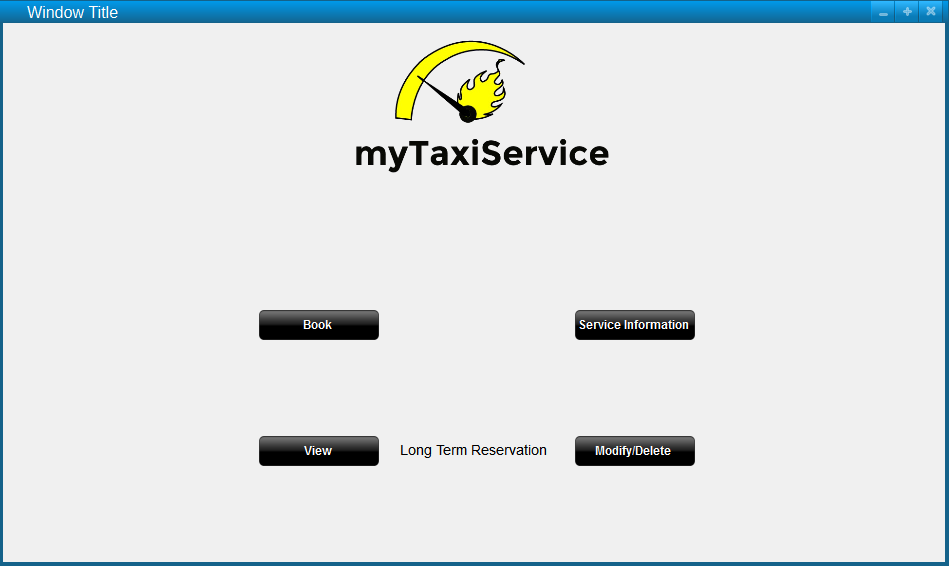
\includegraphics[width=0.90\textwidth]{./images/index}
		\end{center}
		\paragraph{Check Reservation Web Page}
		\begin{center}
			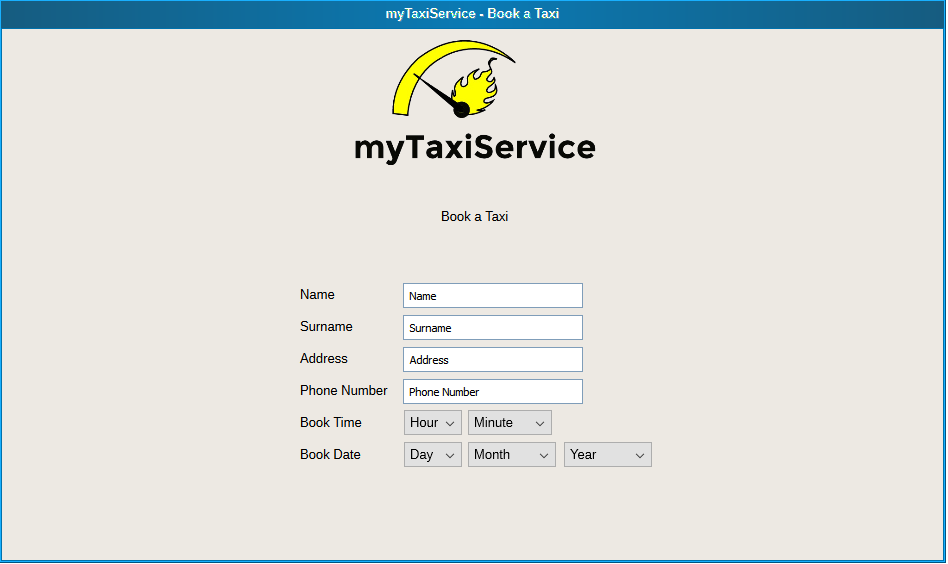
\includegraphics[width=0.90\textwidth]{./images/check_reservation}
		\end{center}
		\paragraph{Modify/Delete Reservation Web Page}
		\begin{center}
			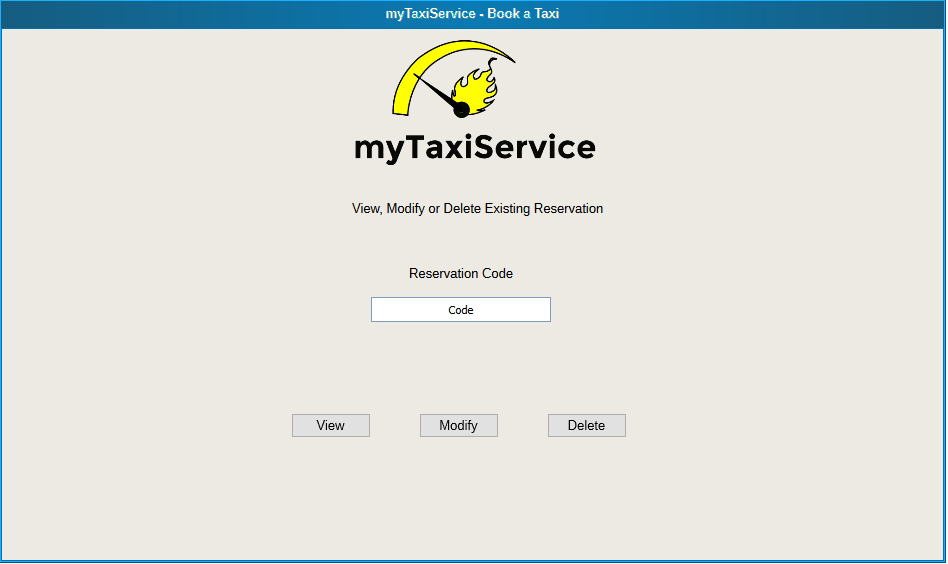
\includegraphics[width=0.90\textwidth]{./images/modify_delete_reservation}
		\end{center}
		\paragraph{Who We Are}
		\begin{center}
			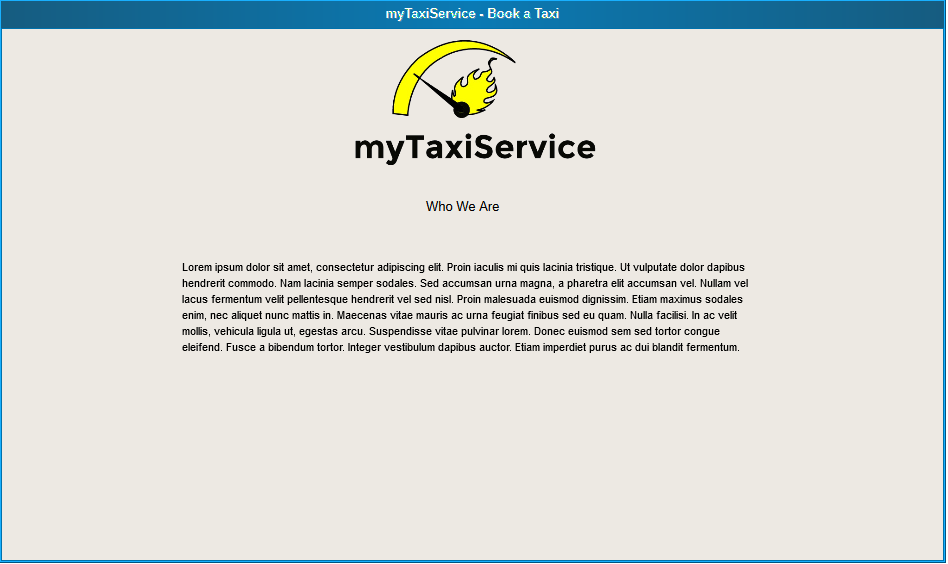
\includegraphics[width=0.90\textwidth]{./images/who_we_are}
		\end{center}
		\subsubsection{Hardware interfaces}
		\begin{itemize}
			\item A machine capable to run a DBMS and a web server software and a PHP interpreter to integrate them
			\item A machine to run the system
			\item Network to connect both machines to one's another and to the Internet
		\end{itemize}
		\subsubsection{Software interfaces}
		\begin{itemize}
			\item A DBMS to store reserved rides data and identifiers of registered Taxis
			\item A web server to provide web pages
			\item A PHP interpreter to integrate the web server and the DBMS
		\end{itemize}
		\subsubsection{Communication interfaces}
		\begin{itemize}
			\item a 
		\end{itemize}
	\subsection{Functional Requirements}
		\subsubsection{Booking a Taxi ride}
		\begin{itemize}
		\item First of all, the system checks the date and the hour of the reservation. 
		\item In case of long-term reservation:
		\begin{enumerate}
		\item the system produces an alphanumeric code;
		\item the system stores this code, with name and surname of the user, in the relative database;
		\item the system assigns this code to the user.
		\end{enumerate}
		\item In case of short-term reservation:
		\begin{enumerate}
		\item the system checks what is the address inserted by the user;
		\item the system checks in which zone of the city is that address, using the GPS information;
		\item the system controls the taxis queue of that zone;
		\item if the taxis queue has at least the identifier of one taxi, the system sends a notification to the first taxi driver of the queue; when it will receive the confirm, the system tells the user that the reservation is been realized;
		\item if the taxis queue hasn't got any taxis identifiers, the system checks the queue of the four adjacent zones of that area; the system continues in this way as long as it finds an available taxi; and then it will do the same things of the \textbf {PUNTO SOPRA}; when the system will receive the confirm, it tells the user that there will be a delay; if the user decides to accept, the system tells him/her that the reservation is been realized, otherwise not.
		\end{enumerate}
		\end{itemize}
		\subsubsection{Update a long-term reservation}
		\begin{itemize}
		\item The system receives the alphanumeric code from the user.
		\item The system checks the DB of the users.
		\item The system displays the information, collected from the DB, to the user.
		\item The system receives the modifications.
		\item The system saves the changed information in the DB.
		\item The system confirms to the user the modifications.
		\end{itemize}
		\subsubsection{Delete a long-term reservation}
		\begin{itemize}
		\item The system receives the alphanumeric code from the user.
		\item The system checks the DB of the users.
		\item The system deletes the found information.
		\item The system confirms to the user the correct elimination.
		\end{itemize}
		\subsubsection{Locate the Users}
		\begin{itemize}
		\item The system takes the address, inserted by the user.
		\item The system searches in which zone of the city is that address, using the GPS information.
		\end{itemize}		
		\subsubsection{Managing Taxis location}
		\subsubsection{Managing Taxi queue}
		\begin{itemize}
			\item A taxi must be free in order to be inserted in a queue
			\item On new rides the system always chose the first taxi in the queue
			\item The queue is managed using a first in, first out policy
			\item Busy taxis are not inserted in any queue
			\item Exists only on queue per zone and it's unique
			\item A queue contains only taxis in the related zone
			\item 
		\end{itemize}
		\subsubsection{Allow Taxi to register in the system}
		\begin{itemize}
			\item A taxi must be not already registered to register his identifier
			\item After the registration the taxi is added to the queue related to the actual zone of the taxi
		\end{itemize}
		\subsubsection{Notify the users about changes about their booking/reservation}
		\begin{itemize}
			\item A user must have requested a taxi ride
			\item One user can only receive only notification about his rides
			\item The system always notifies the user if the taxi is late or becomes not available
		\end{itemize}
		\subsubsection{Notify Taxis about new available rides}
		\begin{itemize}
			\item A taxi must be registered in the system
			\item A taxi must be free to receive a notification
			\item A taxi must confirm or decline the new ride
			\item A taxi only receives notification about his rides
		\end{itemize}
	\subsection{The World and the Machine}
	\begin{center}
		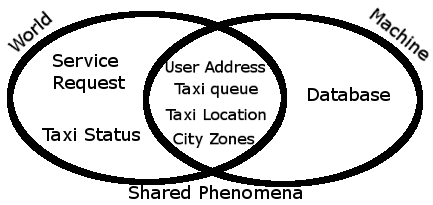
\includegraphics[width=0.85\textwidth]{./images/ellissi}
	\end{center}
	\subsection{Scenarios}
		\subsubsection{Scenario 1}
		Bob has a meeting in Los Angeles two day from now; since he hasn't a car, he decides that he'll call myTaxiService to rent a taxi to take him to the airport. He grabs his cellphone and, with the dedicated app, he books a taxi. The app asks him his name, his surname and where he wants to wait for the taxi. He inserts all the data and, after the server has stored, it notifies Bob that he will receive a notification directly on his phone. The chosen day, 10 minutes before the appointment, the system calls the first free taxi in the nearest zone to the specified location. Unfortunately the first taxi doesn't answer the call so the system puts him at the end of the queue and calls the second one that accepts the assignment and drive Bob to his destination.
		
		\subsubsection{Scenario 2}
		Ann receives a call from one of her friend that tells her that her best friend has given birth to her son, Jimmy. Ann, due to the trains' strike decides to call myTaxiService to take her to the hospital to visit the newborn. So from her pc, she opens www.mytaxiservice.com, goes to the book a taxi section and after she has inserted all the needed data the system tells her that no taxis are available at the moment in the specified zone. Ann that now has become a Desperate Housewife, notice that the system also tells her that a taxi is free from a nearby zone but she has to wait more than the average time for the taxi. Ann decides that waiting up to an hour is not a problem so books the taxi and waits for it. 
		
		\subsubsection{Scenario 3}
		Carl wants to go to visit one of his friends. Using the phone books a taxi. The system then notifies the first taxi in the zone's queue and the taxi confirm the job. Unfortunately a taxi's tyre run flat so the taxi driver has to inform the system that he can't complete the job because a tire is gone, so the system puts him at te end of the queue and calls the second one that accepts the assignment and completes it.
		
		\subsubsection{Scenario 4}
		Thanks to one of his closest friends, Tizio has known a service, called MyTaxiService, that lets to book a taxi, through the web application or the user-friendly mobile one.
		Whereas his computer was broken, using his smart phone, first of all, Tizio has inserted his personal data, that were name, surname and home address. Then, he has chosen the day and the hour for the service. In that moment, the system has received the request of Tizio and it has checked in what zone of the city Tizio was asking for the service. In the taxis queue of that area, the system could have verify that there were no taxis. So it has become to check, starting from the zones near the area in which Tizio has requested a taxi, all the lists of available taxis. 
		Finally the system has found the only one taxi which, in that moment, was available. So the system has sent to Caio the notification of the new route. Besides Caio was standing, with his taxi, in a zone far from the place in which there was Tizio, he has confirmed the service, using the mobile application of his smart phone. After receiving the confirmation, the system has warned Tizio that the taxi would be arrived.
		About one hour later, Tizio is get into the Caio car and so, in a short time, he is arrived in the place where he would have meet his girlfriend Sempronia, relaxing himself, discovering that she was late more than him.

		\subsubsection{Scenario 5}
		Finally, today, Rossana would have taken the airplane. The flight was booked three days ago, but, because of bad weather, it was been deleted. So, she has accessed to the website of MyTaxiService to modify her reservation. She has used her notebook and then she has gone to the web page, concerning the modification/elimination of reservations. In the dedicated form, she has inserted the code that the system gave her to do this stuff, if she would have needed, but she could do it only until twenty minutes before the stipulated time. So she has postponed the reservation, without any problems.
		One hour before the meeting with the taxi, she has received a call from her boyfriend Heric, who wasn't really enthusiastic about her decision to go to USA for the Erasmus. When he has known that Rossana hasn't left yet, Heric has decided to give her a ride to the airport. So the girl, for that moment using her smart phone (the computer was in the luggage), has accessed to the mobile application of MyTaxiService to delete definitely her reservation. Going again in the dedicated page and then inserting her code in the specific form (but now choosing the option "Elimination" from the drop-down list), she has confirmed the cancellation of the reservation. 
		
	\subsection{Non-Functional Requirements}
		\subsubsection{Performance Requirements}
	\subsection{Other requirements}
	